\documentclass[a4paper,11pt]{article}
\usepackage[margin=25mm]{geometry}
\usepackage{fontspec,unicode-math,booktabs,graphicx,array}
\setmainfont{STIXGeneral}\setmathfont{STIX Two Math}
\setlength{\parindent}{0pt}\setlength{\parskip}{5pt}
\begin{document}
\begin{center}{\Large Mixes and graph covers: complete manuscript costs}\\[3pt]
Two originals, both entire common papers, and both complete applications
\end{center}
This comparison enlarges the existing Mixes topic. It retains all 21 pages of
Cunningham and Hubard's mix-criteria article (F005) and all 12 pages of
Leemans and Toledo's faithful-maniplex article (L016). Their corrected principal
contracts have distinct scientific acceptance. The measurement counts two
originals, not their 54 detailed source dispositions.

\textbf{One whole-topic comparison.} The primary coordinate is literal
untrimmed PDF extraction, NFC characters without whitespace. It includes title
matter, abstracts, references, page furniture and arXiv banners on both sides.
\begin{center}\begin{tabular}{lrr}\toprule
Complete manuscript & Pages & Characters\\\midrule
F005 source &21&57753\\
L016 source &12&35506\\
Common simultaneous-action theory $U_0$ &5&12615\\
Common cover theory $U_1$ &4&11641\\
F005 local application $A_1$ &8&20788\\
F005 exceptional application $A_2$ &4&10289\\
L016 application $A_3$ &6&15125\\\bottomrule
\end{tabular}\end{center}
\[
 R_{\mathrm{manuscripts}}=
 \frac{57753+35506}{12615+11641+20788+10289+15125}
 =\frac{93259}{70458}=1.323611.
\]
Both common papers are charged once in this topic. Both F005 papers remain
one complete application, including its exceptional correction. No overlap
is deducted, and no common premise is imported free from another topic.

\textbf{Conditional comparisons.} Only after acquiring \emph{both entire}
common papers, \emph{both whole required finite certificates}, and all retained
mathematical inputs, the individual source/application comparisons are
\[
 r_{\mathrm{F005}}\mid(U,P)=\frac{57753}{20788+10289}
 =1.858384,\qquad
 r_{\mathrm{L016}}\mid(U,P)=\frac{35506}{15125}
 =2.347504.
\]
They do not waive the common acquisition in the whole-topic comparison.
The written replacement is 22801 characters shorter in this primary
representation. This measures manuscript length, not total research effort,
minimum proof complexity or historical originality.

\textbf{Symmetric software boundary.} Optional validation is excluded on
both sides. Neither fixed source contains an executable listing. Their
mathematical tables, formulas, written algorithms and references to software
remain counted. Unprovided historical software has unknown cost. Therefore no
software-inclusive compression factor is calculated; the required programs
remain essential separately disclosed proof inputs, rather than being
reclassified as optional.

\newpage
\begin{center}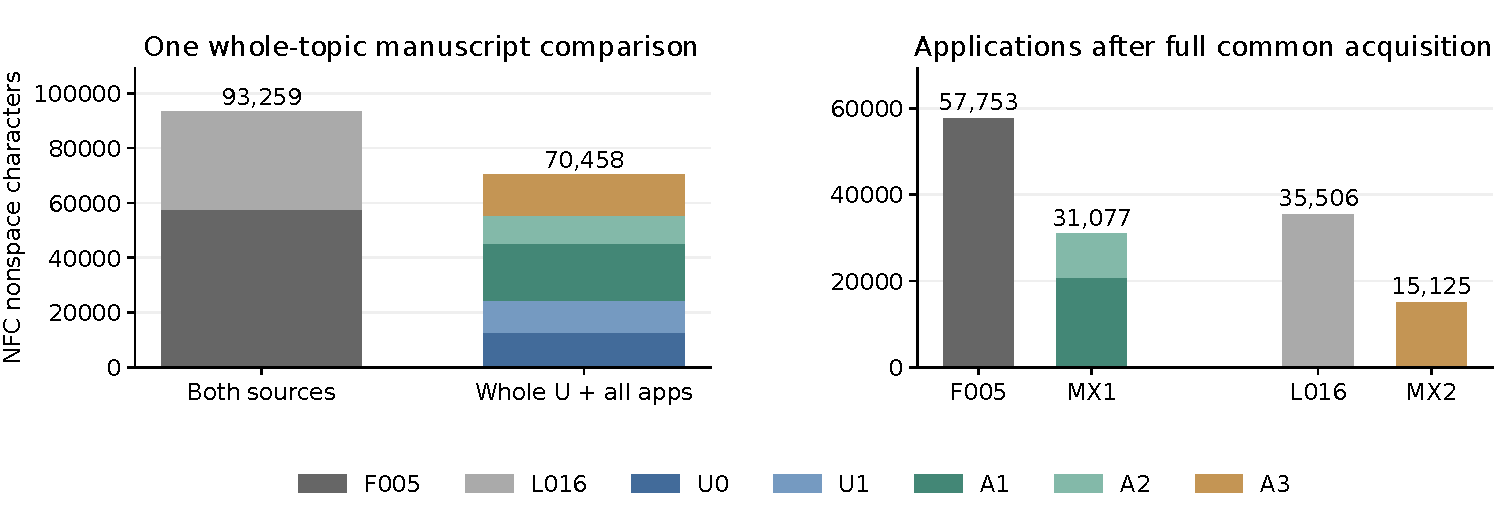
\includegraphics[width=\textwidth]{complete_costs.pdf}\end{center}
Both axes start at zero. The left panel stacks all source and replacement
manuscripts. The right panel shows the two conditional comparisons; its
application bars presuppose the whole common and required-certificate
acquisition. Neither panel charges optional validation on only one side.

\begin{center}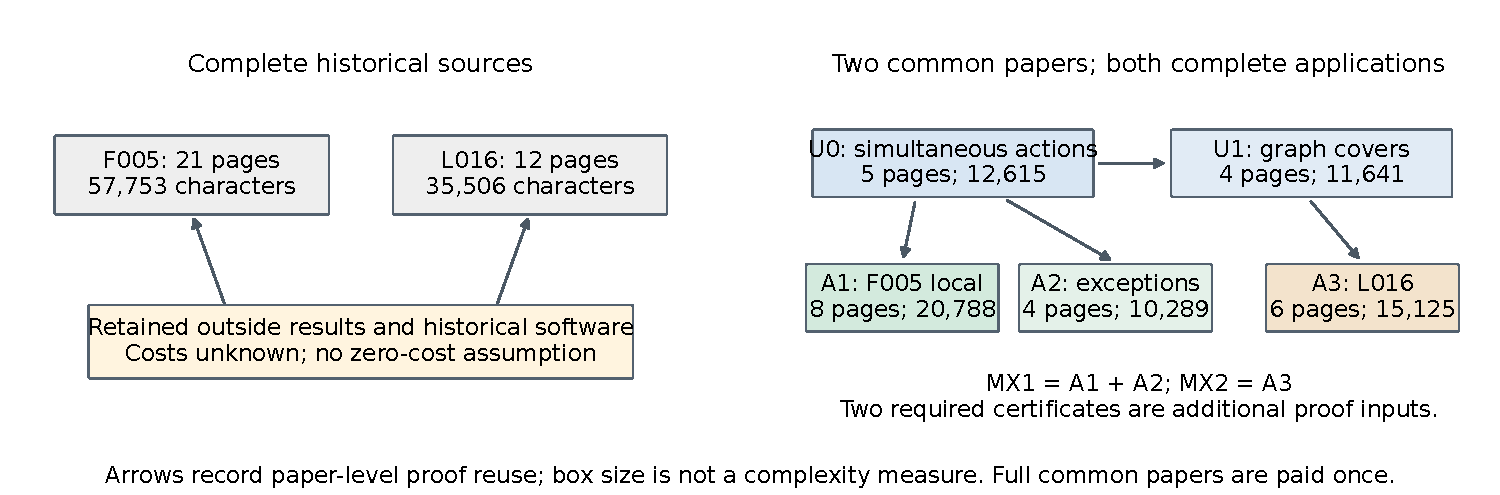
\includegraphics[width=\textwidth]{document_graphs.pdf}\end{center}
The common argument is reused across simultaneous actions and equivariant
graph covers. The paper-level arrows show that reuse, not an exhaustive
historical theorem graph. Every displayed manuscript is counted in full;
box dimensions and node counts are not complexity measures. Required finite
certificates and retained external mathematical inputs remain explicit even
though their full historical costs are unavailable.

\textbf{Scope.} F005 retains its five literal counterexample targets and two
convention-qualified targets, with corrected rooted criteria; its three final
problems remain unanswered. L016's literal Lemma 3.5 is disproved and repaired
under faithfulness. Proposition 5.4 correctly says \emph{without} the component
intersection property. Its principal families and rank-three result are
recovered; ancillary smallest/atlas counts and further-cover questions remain
outside that contract. These qualifications do not prune either full source.

\newpage
\section*{Whole programs and representation limits}
The two required finite certificates are the complete
\texttt{check\_coprime.g} and \texttt{base\_certificate.g}. Their raw primary
cost is 2907 characters; the complete two-page printed alternative costs
3431. Printed and raw versions represent the same files and are never added
together. The source-side counterpart remains unknown, so neither inventory
produces an additional ratio.
\begin{center}\begin{tabular}{lrr}\toprule
Separate complete raw-file inventory &Files&Characters\\\midrule
Required finite certificates &2&2907\\
Optional validation &4&19467\\
Operational drivers &5&21999\\
Scoped Lean files &2&4181\\\bottomrule
\end{tabular}\end{center}
All four optional files remain visible. The three-page new optional appendix
costs 7285 characters; the two old mixed appendices cost 8813 and
7212 and remain historical inventories. They are not extra required
charges or current optional-inclusive comparisons. The two Lean files provide
six generic declarations, four new and two reused. They do not formalize all
geometry, the finite presentations or either complete source.

\textbf{Unit sensitivity.} Complete untrimmed extraction under NFC gives:
\begin{center}\small\begin{tabular}{lrrr}\toprule
Unit&Whole topic&F005 conditional&L016 conditional\\\midrule
Whitespace tokens & 1.497 & 2.026 & 2.784 \\
Alphanumeric runs & 1.505 & 2.064 & 2.766 \\
Nonspace characters & 1.324 & 1.858 & 2.348 \\
Collapsed-space characters & 1.355 & 1.889 & 2.424 \\
Collapsed-space UTF-8 bytes & 1.279 & 1.775 & 2.309 \\
\bottomrule\end{tabular}\end{center}
The JSON and CSV retain all five units under NFC and NFKC in raw-untrimmed,
raw-selected and calibrated-selected forms: 30 coordinates and 90 exact
fractions. Selection removes only the separately bound running headers and
isolated folios. Calibration changes declared visible glyph representations,
including script letters, brace pieces and arrow-tee components; the original
raw extraction always remains available. Literal line-break hyphens remain.

All 180 earlier F005 PDF cells and 70 raw-file cells are retained exactly.
The new five-document input contributes 150 PDF cells and 60 raw-file cells.
The combined eleven-document inventory includes historical code PDFs and
therefore is \emph{not} a list of eleven denominator terms. The current
manuscript denominator contains exactly the two common papers and three
application papers shown on page 1.

Diagram labels are retained when extractable. Full graphic/layout cost,
retained outside proofs, original software, runtime, engineering and complete
formalization remain unknown rather than zero. Distinct input acceptance is
bound; this numerical author packet still requires a separate arithmetic,
graph and reader review. It creates no new source, question or novelty credit.
\end{document}
